\chapter{Конструкторская часть}\label{ch:-3}

В данном разделе будут приведены описания алгоритмов решения задачи коммивояжера, а также модель вычисления трудоемкости алгоритмов.


\section{Описание алгоритмов}\label{sec:-3}
На вход алгоритмов подается информация о графе в виде матрицы связности $M$.
Для муравьиного алгоритма дополнительно задаются следующие параметры:
\begin{itemize}
    \item максимальное число итераций $t_{\text{max}}$,
    \item количество муравьёв $N_{\text{ants}}$,
    \item коэффициент влияния феромона $\alpha$,
    \item коэффициент испарения феромона $\rho$,
    \item бюджет ресурсов $\text{max\_resources}$.
\end{itemize}

На выходе -- длина наилучшего маршрута $L_{best}$ и сам маршрут в виде массива вершин.

На схемах~\ref{scheme:brf}---~\ref{scheme:updpher} приведены описания алгоритмов решения задачи коммивояжера: алгоритм полного перебора, муравьиный алгоритм.

\clearpage

\begin{figure}[H]
    \centering
    
\includegraphics[scale=0.65]{images/s1}
    \caption{Описание алгоритма полного перебора}
    \label{scheme:brf}
\end{figure}

\clearpage

\begin{figure}[H]
    \centering
    
\includegraphics[scale=0.65]{images/s2}
    \caption{Описание муравьиного алгоритма}
    \label{scheme:antbeg}
\end{figure}

\clearpage

\begin{figure}[H]
    \centering
    
\includegraphics[scale=0.8]{images/s3}
    \caption{Описание муравьиного алгоритма -- нахождение вероятностей}
    \label{scheme:antprob}
\end{figure}

\begin{figure}[H]
    \centering
    
\includegraphics[scale=0.65]{images/s4}
    \caption{Описание муравьиного алгоритма -- выбор следующего города}
    \label{scheme:antchoose}
\end{figure}

\clearpage

\begin{figure}[H]
    \centering
    
\includegraphics[scale=0.8]{images/s5}
    \caption{Описание муравьиного алгоритма -- выбор лучшего решения}
    \label{scheme:antchooseres}
\end{figure}

\clearpage

\begin{figure}[H]
    \centering
    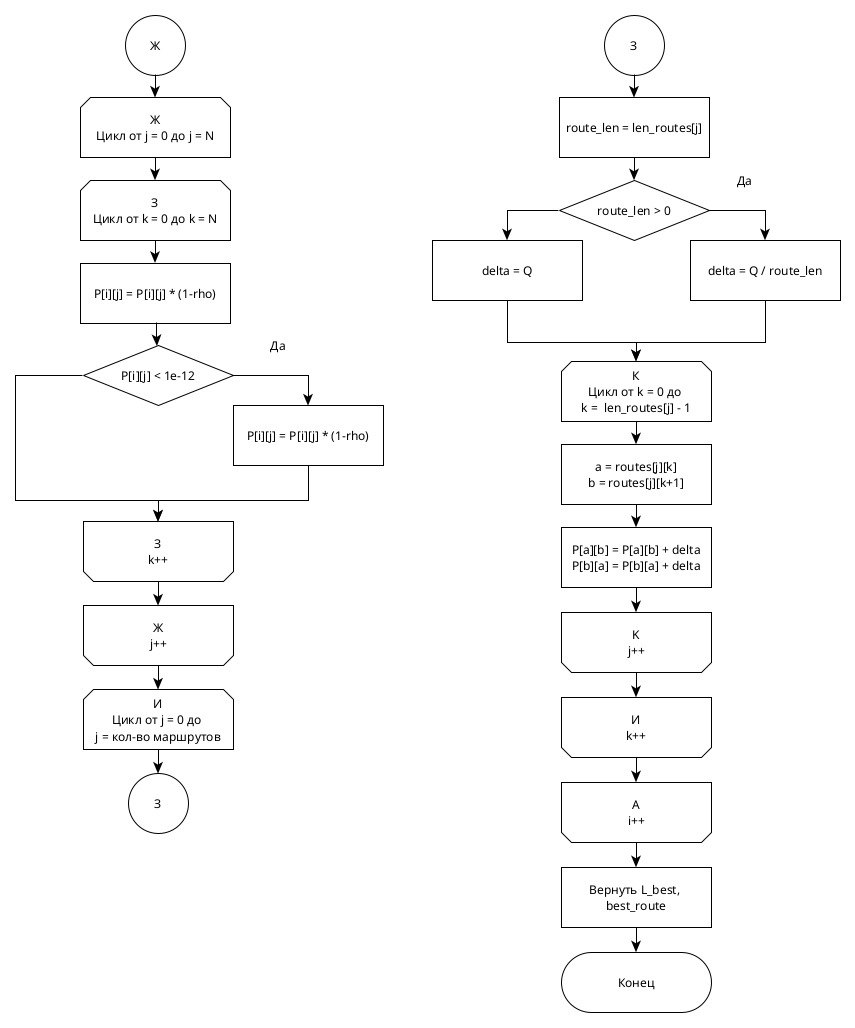
\includegraphics[scale=0.55]{images/s6}
    \caption{Описание муравьиного алгоритма -- обновление феромонов}
    \label{scheme:updpher}
\end{figure}

\clearpage


\section{Модель вычислений}

Для вычисления трудоемкостей алгоритмов необходимо ввести модель вычислений:

\begin{itemize}
    \item операции $+, -, [], ++, {-}-, ==, !=, <, >, <=, >=$ имеют трудоемкость 1;
    \item операции $*, /, \%, /=,  *=, \%=$ имеют трудоемкость 2;
    \item трудоемкость условного оператора \text{if <condition> then A else B} рассчитывается, как (\ref{eq:ifcond});
    \begin{equation}
        \label{eq:ifcond}
        f_{if} = f_{\text{condition}} +
        \begin{cases}
            f_A, & \text{если условие выполняется,}\\
            f_B, & \text{иначе.}
        \end{cases}
    \end{equation}
    \item трудоемкость цикла \text{for (init; condition; increment) \{ body \}} рассчитывается, как (\ref{eq:forcyc});
    \begin{equation}
        \label{eq:forcyc}
        f_{for} = f_{\text{init}} + f_{\text{condition}} + N\cdot(f_{\text{body}} + f_{\text{condition}} + f_{\text{increment}})
    \end{equation}
    где N -- количество итераций цикла;
    \item трудоемкость вызова функции равна 0.
\end{itemize}


\section{Вычисление трудоемкости алгоритмов}

Далее представлен расчет трудоемкостей алгоритмов.
Для расчета представлены такие алгоритмы, как алгоритм полного перебора и муравьиный алгоритм.

Проверка входных данных и инициализация массива лучшего маршрута $best\_route$ и длины $L_{best}$ в расчетах учитываться не будут, так как данные действия не являются самыми трудоемкими и являются общими для всех алгоритмов.

Обозначения размерностей:

\begin{itemize}
    \item $N$ -- размерность матрицы смежности;
    \item $M$ -- количество муравьев;
    \item $T_{max}$ -- количество итераций.
\end{itemize}

\subsection{Алгоритм полного перебора}

Расчет трудоемкости стандартного алгоритма:

\begin{itemize}
    \item трудоемкость генерации всех перестановок, $f_{perm} = N! \cdot N$;
    \item трудоемкость внешнего цикла по перестановкам, $f_{i} = 3 + N! \cdot (2 + f_{body_{i}})$;
    \item трудоемкость цикла по вершинам графа, $f_{j} = 3 + (N-1) \cdot (3 + f_{sum})$;
    \item трудоемкость суммирования меток, $f_{sum} = 7$.
\end{itemize}

Трудоемкость проверки на лучший маршрут~\ref{eq:cmp}:

\begin{equation}
    \label{eq:cmp}
    f_{cond} =
    \begin{cases}
        1, & \text{длина маршрута больше или равна лучшего(л.с.),}\\
        3, & \text{иначе (х.с.).}
    \end{cases}
\end{equation}

Итоговая трудоемкость:

$f_{brf} = N! \cdot N + 3 + N!(2 + 1 + 3 + (N-1) \cdot 7 + 1)$ -- л.с.

$f_{brf} = N! \cdot N + 3 + N!(2 + 1 + 3 + (N-1) \cdot 7 + 3)$ -- х.с.

После приведения:

\begin{equation}
    \label{eq:ansbrf}
    f_{brf} =
    \begin{cases}
        N! \cdot 8N + 3, & \text{(л.с.),}\\
        N! \cdot (8N + 2) + 3, & \text{(х.с.),}
    \end{cases}
\end{equation}

\subsection{Муравьиный алгоритм}

Расчет трудоемкости муравьиного алгоритма:

\begin{itemize}
    \item сложность инициализации начальных параметров пренебрежимо мала, $f_{1} = 1$;
    \item инициализация квоты феромона $F_{Q} = 2N$;
    \item инициализация матрицы феромонов $F_{P} = N^2$;
    \item инициализация эвристической матрицы $F_{eta} = N^2$;
    \item сложность основного цикла по итерациям $f_{main} = 2 + T_{max} \cdot (2 + f_{bodyT})$;
    \item сложность внутреннего цикла по муравьям $f_{ants} = 2 + M \cdot (2 + f_{bodyA})$.
\end{itemize}

Расчет сложности по телу цикла $f_{ants}$, инициализация:

$f_{2} = 3 + N + 2 + 2 + 1 + 1 = 9 + N$.

Поиск вероятностей:

$f_{3} = 2 + N \cdot (2 + N \cdot (2 + 2 + 3 + 2 + 11 + 2) + 1 + N + 2 + 1 + 1 + f_{nextC}) = 2 + N \cdot(23N + 7 + f_{nextC})$.

Поиск следующего города:

$f_{nextC} = 2 + \frac{N}{2}(2 + 3 + 3 + 2) + 2 + 2 + 3 + 2 + 1 = 5N + 12$.

Суммарная сложность цикла обхода городов:

$f_{3} = N + 2 + N \cdot (23N + 7 + 5N + 12) = 27N^2 + 20N + 2$.

Обновление результата:

$f_{upd} = 1 + 7(N-1) + 4 + 2 = 7N$

Суммарная сложность цикла по муравьям:

$f_{ants} = 2 + M \cdot (2 + f_{2} + f_{3} + f_{upd}) = 2 + M \cdot (2 + 9 + N + 27N^2 + 20N + 2 + 7N) = 2 + M \cdot (27N^2 + 28N + 13)$

Обновление феромонов:

$f_{pher} \approx N^2$

Нанесение феромонов:

$f_{pher2} \approx N * M$

Результирующая трудоемкость муравьиного алгоритма:

$f_{Aans} = 1 + 2N + N^2 + N^2 + 2 + T_{max} \cdot (2 + 2 + M \cdot(27N^2 + 28N + 13) + N^2 + N*M) \approx 27T_{max} \cdot MN^2 \approx 27N^4$

\section*{Вывод}
В данном разделе были представлены схемы алгоритмов решения задачи коммивояжера, а также оценены трудоемкости для данных алгоритмов.
Алгоритм полного перебора имеет большую трудоемкость по сравнению с муравьиным.

